


\begin{document}
The base level schematic or block diagram is shown below in Figure \ref{fig:blockproposal}.
\begin{figure}
	\centering
	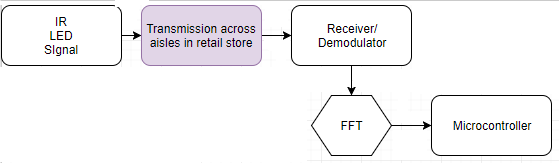
\includegraphics[width=0.7\linewidth]{Proposed_work/blockproposal}
	\caption{System level schematic of foot-traffic sensor}
	\label{fig:blockproposal}
\end{figure}

The optical uplink has the transmitter and receiver already constructed. The transmitter and receiver will transmit information to the microcontroller, which will count the amount of foot traffic in retail stores. 

The actual sensor will require a pair of parallel beams, placed at waist height at the entrance and exit of each aisle. The reasoning for the parallel beams is that it would enable the microcontroller to calculate which direction foot traffic flows, entering or exiting the aisles. There are limitations with regards to density of traffic, where the beams may be blocked for a longer duration, counting only one person when there are multiple in reality. Algorithms will take this into account within the microcontroller as to not negatively impact the data. The circuit will be powered by a 9V source, and will output a constant infrared during store hours. As a person moves through the parallel beams, the microcontroller will process the lack of the beams, detecting which was interrupted first, then save the data to the DRAM. 



\end{document}